\documentclass[11pt]{article}

%{{{ Packages
\usepackage[margin=1in]{geometry}
\usepackage{enumitem}
\usepackage{amsfonts}
\usepackage{amssymb}
\usepackage{amsmath}
\usepackage{amsthm}
\usepackage{mathdots}
\usepackage{mathtools}
\usepackage[dvipsnames]{xcolor}
\usepackage[framemethod=TikZ]{mdframed}
\usepackage{microtype}
\usepackage{witharrows}
\usepackage{float}
\setlength{\parindent}{0pt}
%}}}
%{{{ Custom commands
% Nice maths commands
\newcommand{\defeq}{:=}
\newcommand{\eqdef}{+:}
\newcommand{\abs}[1]{|#1|}
\newcommand{\norm}[1]{||#1||}
%\renewcommand{\dots}{...}
\newcommand{\msrspc}{\ensuremath{(X,\mathcal{A},\mu)}}
\newcommand{\sigal}{$\sigma$-algebra}
\newcommand{\relmiddle}[1]{\mathrel{}\middle#1\mathrel{}}
\newcommand{\rmv}{\relmiddle|}
\newcommand{\dm}{\ensuremath{\,d\mu}}
\DeclareMathOperator\vol{vol}
\newcommand{\stcmp}{^{\mathsf{c}}}

% Spaces
\newcommand{\pow}[1]{\mathcal{P}(#1)}
\newcommand{\ktor}{\mathbb{T}^k}
\newcommand{\R}{\mathbb{R}}
\newcommand{\Rb}{\overline{\R}}
\newcommand{\C}{\mathbb{C}}
\newcommand{\Z}{\mathbb{Z}}
\newcommand{\N}{\mathbb{N}}
\newcommand{\Q}{\mathbb{Q}}

% Derivatives
\newcommand*{\pd}[3][]{\ensuremath{\frac{\partial^{#1} {#2}}{\partial {#3}^{#1}}}}
\newcommand{\grad}{\bigtriangledown}

% Vectors
\newcommand{\mv}[1]{\textbf{#1}}

%}}}
%{{{ Enviornments
% Definitions environment
\newenvironment{defin}
	{\begin{mdframed}[backgroundcolor=white, roundcorner=5pt, linewidth=1pt]}
	{\end{mdframed}}
\newcommand{\mdf}[1]{{\color{red} #1}}

% Important notes environment
\newenvironment{note}
	{\begin{mdframed}[backgroundcolor=white, linecolor=red, roundcorner=5pt, linewidth=1pt]\bfseries{Note:}\normalfont}
	{\end{mdframed}}

% Examples enviornmnet
\definecolor{mylg}{rgb}{0.9,0.9,0.9}
\newenvironment{eg}
	{\begin{mdframed}[backgroundcolor=myld,roundcorner=5pt,linewidth=0pt]\bfseries{Example:}}
	{\end{mdframed}}

% Theorem enviornment
\newtheorem{theorem}{Theorem}[section]
\newtheorem{prop}[theorem]{Proposition}
\newtheorem{cor}[theorem]{Corollary}
%}}}
%{{{ Document metadata
\title{Measure Theory - Overview}
\author{}
\date{}
%}}}

\begin{document}
\maketitle
\section{Starting definitions}
\begin{defin}
Start with a set $X$.
$\mathcal{A}\subseteq\pow{X}$ is called an \mdf{algebra} if 
\begin{itemize}
	\item $\mathcal{A}$ is non-empty
	\item $X\in \mathcal{A}$
	\item $\mathcal{A}$ is closed and under complementation
	\item $\mathcal{A}$ is closed under finite unions and intersections
\end{itemize}
We obtain a \mdf{\sigal} if we also have closure under countable unions and intersections.
We say a set $A\in\mathcal{A}$ is \mdf{$\mathcal{A}$-measurable}.
\end{defin}
Note that intersecting {\sigal s} obtains a new {\sigal} but taking unions does not necessarily work.
A very important {\sigal} is the \mdf{Borel \sigal},
$$\mathcal{B}(\R^d)\defeq\sigma\left(\{\text{open sets in }\R^d\}\right)$$
Note that it can also be formed by all closed sets, closed half-rays or half-open intervals.
\begin{defin}
	Given a {\sigal} $\mathcal{A}$ on a set $X$, a \mdf{measure} on $(X,\mathcal{A})$ is a function $\mu:\mathcal{A}\to[0,+\infty]$ such that
	\begin{itemize}
		\item $\mu(\emptyset)=0$
		\item Given disjoint $A_1,A_2,\dots\in\mathcal{A}$,
			$$\mu\left(\bigcup_{i=1}^\infty A_i\right)=\sum_{i=1}^\infty \mu(A_i)$$
	\end{itemize}
	This gives us a \mdf{measure space} \msrspc.
	
	We call this measure \mdf{finite} if $\mu(X)<\infty$ and \mdf{$\sigma$-finite} if we can write $X$ as a union of finite measure sets.
\end{defin}
Note measures are always increasingly monotonous and countably sub-additive.
We also have the following very important property:
\begin{prop}[Continuity of measure]
	Given a measure space \msrspc.
	\begin{itemize}
		\item $A_1\subseteq A_2\subseteq \dots$ in $\mathcal{A}$ then
			$$\mu\left(\bigcup_i A_i\right)=\lim_i\mu(A_i)$$
		\item $A_1\supseteq A_2\supseteq \dots$ in $\mathcal{A}$ then
			$$\mu\left(\bigcap_k A_k\right)=\lim_k \mu(A_k)$$
	\end{itemize}
\end{prop}
A very important measure is the Lebesgue measure since it coincides with our natural intuition for the measure of subsets of $\R^d$.
First we need to define an outer measure.
\begin{defin}
	An \mdf{outer measure} is a function $\mu^*:\pow{X}\to[0,+\infty]$ such that
	\begin{itemize}
		\item $\mu^*(\emptyset)=0$
		\item $A\subseteq B\subseteq X\implies \mu^*(A)\leq\mu^*(B)$
		\item Given a countable collection of subsets $A_i\subseteq X$, we have countable sub-additivity 
			$$\mu^*\left(\bigcup_i A_i\right)\leq\sum_i \mu^*(A_u)$$
	\end{itemize}
	Notably we require monotonicity as an axiom and also require that the outer measure is defined on every subset.
	This is a weaker notion than a measure.

	Given $A\subseteq\R$, $\mathcal{C}_A\defeq\left\{\text{Collections}\;\{(a_i,b_i)\}_{i=1}^\infty \rmv -\infty < a_i < b_i < \infty, \; \cup_{i=1}^\infty (a_i,b_i)\supseteq A \right\}$.
	This is the set of collections of finite open intervals which cover the set A.
	We can then define the \mdf{Lebesgue outer measure} on $A$ to be
	$$\lambda^*(A)\defeq\inf\left\{\sum_i(b_i-a_i) \rmv \{(a_i,b_i\}_{i=1}^\infty\in\mathcal{C}_A\right\}$$
\end{defin}
\begin{prop}
	$\lambda^*$ is an outer measure on $\R$ and $\lambda^*([a,b])=b-a$, $\forall a, b\in\R$ such that $a\leq b$.
\end{prop}
\begin{proof}
The only difficult things to prove are countable sub-additivity and the desired value for intervals.
\begin{enumerate}[label=(\roman*)]
	\item Given $A_1,A_2, \dots\subseteq\R$ we may assume that $\lambda^*(A_i)<\infty$ for all $i$ else countable sub-additivity holds trivially.
		Given $\epsilon >0$ we can pick $\left\{(a_{i_n},b_{i_n})\right\}_{i=1}^\infty\in\mathcal{C}_{A_i}$ such that 
		$$\sum_{n=1}^\infty (b_{i_n}-a_{i_n})< \lambda^*(A_i)+\frac{\epsilon}{2^i}$$
		We can union these countably many countable collections to get another countable collection covering $\cup_i A_i$.
		\begin{align*}
			\lambda^*\left(\bigcup_i A_i\right)&\leq \sum_j(b_j-a_j)\\
											   &=\sum_i\left(\sum_n\left(b_{i_n}-a_{i_n}\right)\right)\\
											   &\leq\sum_i\left(\lambda^*(A_i)+\frac{\epsilon}{2_i}\right)\\
											   &\leq\left(\sum_i\lambda^*(A_i)\right)+\epsilon
		\end{align*}
		Taking $\epsilon\to 0$ yields the result.
	\item Just think of a nice cover than does the job either exactly or to within $\epsilon$, depending on your philosophy surrounding the set $\mathcal{A}$.
\end{enumerate}
\end{proof}
By taking $d$-dimensional `rectangular' intervals we can use the same procedure to define a Lebesgue measure on $\R^d$ which similarly assigns expected `volumes' to these rectangles.
The proof of this is somewhat more involved.
Now for a weird definition.
\begin{defin}
Given an outer measure $\mu^*$ on $X$, $B\subseteq X$ is \mdf{$\mu^*$-measurable} if
\[
	\forall A \in \pow{X} \quad \mu^*(A)=\mu^*(A\cap B)+\mu^*(A\cap B\stcmp)
\]
Intuitively, $B$ is `nice' if when we want to measure any other set we just measure the part inside and the part outside $B$ and then add the measures together.
\end{defin}
It's easy to show that any set with zero outer measure or who's complement has zero outer measure is outer measurable.
Define 
\[
	M_{\mu^*}\defeq\left\{\mu^*\text{-measurable sets}\right\}
\]
\begin{theorem}
	Given an outer measure $\mu^*$, $M=M_{\mu^*}$ is a {\sigal} and $\mu^*$ yields a measure when restricted to $M_{\mu^*}$.
\end{theorem}
\begin{proof}
We certainly have $\sigma,X\in M$ and closure under complementation.
First lets prove closure under finite union.
Take $B_1,B_2\in M$ and choose $A\subseteq X$ arbitrary.
\[
	\begin{WithArrows}
		& \mu^*(A\cap(B_1\cup B_2))+\mu^*(A\cap(B_1 \cup B_2)\stcmp)\Arrow{$B_1$ measurable} \\
		&=\mu^*\left[(A\cap(B_1\cup B_2))\cap B_1\right]+\mu^*\left[(A\cap(B_1\cup B_2))\cap B_1\stcmp\right]\\
		&\quad+\mu^*\left[A\cap (B_1\cap B_2)\stcmp\right]\Arrow{simplify sets}\\
		&=\mu^*(A\cap B_1) + \mu^*(A\cap B_1\stcmp \cap B_2) + \mu*(A\cap B_1\stcmp \cap B_2\stcmp)\Arrow{$B_2$ measurable}\\
		&=\mu^*(A\cap B_1) + \mu^*(A\cap B_1\stcmp)\Arrow{$B_1$ measurable}\\
		&=\mu^*(A)
	\end{WithArrows}
\]
So $M$ is certainly an algebra. To obtain countable unions we note the following can be proved by induction.
Given $B_1, B_2,\dots\in M$ and any $A\subseteq X$.
\[
	\mu^*(A)=\sum_{i=1}^n\mu^*(A\cap B_i)+ \mu^*\left(A\cap\left(\bigcup_{i=1}^n B_i\right)\stcmp\;\right)\quad\forall n\in\N
\]
Letting $n\to\infty$, by monotonicity of the outer measure on right term we get
\[
	\begin{WithArrows}
		\mu^*(A)&\geq \underbrace{\sum_{i=1}^\infty \mu^*(A\cap B_i)}_{\text{converges since all terms +ve}}+\mu^*\left(A\cap\left(\bigcup_{i=1}^\infty B_i\right)\stcmp\right)\Arrow{sub-additivity}\\
				&\geq \mu^*\left(A\cap \left(\bigcup_{i=1}^\infty B_i\right)\right)+\mu^*\left(A\cap\left(\bigcup_{i=1}^\infty B_i\right)\stcmp\;\right)
	\end{WithArrows}
\]
and hence $\cup_i B_i \in M$ because the other inequality is an axiomatic assumption.
For arbitrary sets we can just take appropriate complementation to express their union as a union of pairwise disjoint sets.

It remains to show that we get a measure.
Again the only thing to really show is the remaining inequality to get countable additivity.
Given disjoint $B_1, B_2, \dots$ in $M$ just take $A=\cup_i B_i$ in the above inequality to get
\[
	\mu^*\left(\bigcup_{i=1}^\infty B_i\right)\geq \sum_{i=1}^\infty \mu^*(B_i) + \mu^*(\emptyset)
\]
\end{proof}

\subsection{Working with Lebesgue Measures}
We are now able to form a measure from the Lebesgue outer measure.
\begin{defin}
	The \mdf{Lebesgue measurable sets} are exactly the $\lambda^*$-measurable sets.
	The resulting {\sigal} is denoted $\mathcal{L}^d$.
	Restricting $\lambda^*$ to $\mathcal{L}^d$ yields the \mdf{Lebesgue measure} $\lambda_d$.
\end{defin}
\begin{prop}
	\[
		\mathcal{B}(\R^d)\subseteq\mathcal{L}( \R^d)
	\]
\end{prop}
\begin{proof}
Take $b\in\R$, we will show that $(-\infty, b]\in\mathcal{L}$ so that we can take $\sigma$ on either side to obtain the result.
Pick any $A\subseteq\R$ such that $\lambda^*(A)<\infty$ and take arbitrary $\epsilon >0$.

Choose $\left\{(a_i, b_i)\right\}\in\mathcal{C}_A$ such that $\sum_i (b_i - a_i) < \lambda^*(A) + \epsilon$.
Notice that $(a_i, b_i)\cap B$ and $(a_i, b_i)\cap B\stcmp$ are disjoint intervals whose lengths sum to $b_i - a_i$.
\[
	\begin{WithArrows}
		&\quad\;\lambda^*(A\cap B) + \lambda^*(A\cap B\stcmp) \Arrow{monotoncity} \\
		&\leq \lambda^*\left(\left[\cup_i(a_i, b_i)\right]\cap B\right) + \lambda^*\left(\left[\cup_i(a_i, b_i)\right]\cap B\stcmp\right) \Arrow{countable sub-additivity} \\
		&\leq\sum_i\lambda^*((a_i, b_i)\cap B) + \sum_i \lambda^*((a_i, b_i)\cap B\stcmp) \Arrow{rearrange +ve terms}\\
		&\leq \sum_i\left[\text{length}\left((a_i, b_i)\cap B\right) + \text{length}\left((a_i, b_i)\cap B\stcmp\right)\right]\\
		&=\sum_i (b_i - a_i) < \lambda^*(A) + \epsilon
	\end{WithArrows}
\]
Now taking $\epsilon\to 0$ we obtain the troublesome inequality.
\end{proof}
It is often useful to be able to approximate the Lebesgue measure from above and from below.
\begin{prop}[Regularity of Measure]
	Let $A\in\mathcal{L}(\R^d)$ then
	\begin{enumerate}[label=(\alph*)]
		\item $\lambda(A)=\inf\left\{\lambda(U) \rmv U\;\text{open}\;,U\supseteq A\right\}$
		\item $\lambda(A)=\sup\left\{\lambda(K) \rmv  K\;\text{compact}\;,K\subseteq A\right\}$
		\item $\text{RHS}(a)=\text{RHS}(b)\implies A\in\mathcal{L}(\R^d)$
	\end{enumerate}
\end{prop}
\begin{proof}
Every measure is monotonous so we only have one inequality to prove in each case.
\begin{enumerate}[label=(\alph*)]
	\item Assume $\lambda(A)< \infty$ else we are already done.
		Given any $\epsilon>0$, pick $\left\{R_i\right\}\in\mathcal{C}_A$ such that $\sum_i\vol(R_i)\leq\lambda^*(A)+\epsilon < \lambda(A) + \epsilon$.
		Define $U\defeq\cup_i R_i$ which is then an open set such that $A\subseteq U$.
		Now we have
		\[
			\lambda(U)\leq\sum_i\lambda(R_i)=\sum_i\lambda^*(R_i)=\sum_i\vol(R_i)\leq\lambda(A)+\epsilon
		\]
		Taking $\epsilon\to 0$ yields the result
	\item Again take $\epsilon >0$ arbitrarily, we split into cases.

		\textbf{Case 1:} A is a bounded set.

		Take $C\supseteq A$ which is compact. Now by $(a)$ there is $U$ open with $U\supseteq C\setminus A$ such that
		\[
			\lambda(U) \leq \lambda(C\setminus A) + \epsilon
		\]
		Now define $K\defeq C\setminus U$.
		Then $C$ is closed and $U$ is open so $K$ is closed and $K$ lives within $C$ so is bounded.
		Hence $K$ is bounded.
		Also note $K\subseteq A$.
		\begin{align*}
			\lambda(C)&\leq\lambda(K)  + \lambda(U) \\
					&\leq \lambda(K) + \lambda(C\setminus A) + \epsilon
		\end{align*}
		Hence
		\[
			\lambda(K)\geq \lambda(C) - \lambda(C\setminus A) - \epsilon = \lambda(A) - \epsilon
		\]
		Taking $\epsilon\to 0$ yields $\sup\geq \lambda(A)$.

		\textbf{Case 2:} A is an unbounded set.

		The issue this time is we can't really choose that $C$.
		This time define $A_i\defeq A \cap [-i, i]^d$ and set $A\defeq\cup_i A_i$ to see
		\[
			A_1 \subseteq A_2 \subseteq A_3 \subseteq \dots
		\]
		Continuity of measure tells us that $\lim_{n\to\infty}\lambda (A_i)=\lambda (A)$.
		So given $\epsilon >0$ there is $n\in\N$ such that $\lambda (A_n)\geq \lambda (A) - \frac{\epsilon}{2}$.
		Case 1 tells us that there is compact $K$ such that $K\subseteq A_n\subseteq A$ with the property that
		\[
			\lambda(K)\geq\lambda(A_n)-\frac{\epsilon}{2}\geq\lambda(A) - \epsilon
		\]
		Taking $\epsilon\to 0$ yields our result.
\end{enumerate}
\end{proof}
One nice property of the Lebesgue measure is translation invariance.
\begin{prop}[Translation invariance]
	Fix $x\in\R^d$ then
	\begin{enumerate}[label=(\alph*)]
		\item $\forall A\in\pow{\R^d}\quad\lambda^*(A)=\lambda^*(A+x)$
		\item $A\in\mathcal{L}\implies A+x\in\mathcal{L},\quad \lambda(A+x)=\lambda(A)$
	\end{enumerate}
\end{prop}
\begin{proof}
\begin{enumerate}[label=(\alph*)]
	\item Given a covering collection $\left\{(a_i, b_i)\right\}\in\mathcal{C}_A$ we can just translate these intervals and the volume is preserved.
	\item We first show that $A+x$ is $\lambda^*$-measurable. 
		\[
			\begin{WithArrows}
			&\quad\;	\lambda^*(B\cap (A+x)) + \lambda^*(B\cap (A+x)\stcmp)\Arrow{using (a)}\\
			&= \lambda^*((B-x)\cap A) + \lambda^*((B-x) \cap A\stcmp)\Arrow{$A\in\mathcal{L}$}\\
			&=\lambda^*(B-x)\Arrow{using (a)}\\
			&=\lambda^*(B)
			\end{WithArrows}
		\]
		and hence $A+x\in\mathcal{L}$.
		Also $\lambda(A+x)=\lambda^*(A+x)=\lambda^*(A)=\lambda(A)$.
\end{enumerate}
\end{proof}
The question arises whether there exists a set which cannot be measured by the omnipotent Lebesgue.
This depends on your view of the Axiom of Choice.
\begin{theorem}[Vitali Set]
	Assuming the axiom of choice, $\exists E\subseteq (0, 1)$ such that $E\not\in\mathcal{L}(\R)$.
\end{theorem}
\begin{proof}
Can't be bothered to do this atm.
\end{proof}
\section{Extended Real Line}
We can extend the real line by adding two points
\[
	\Rb\defeq\R\cup\left\{-\infty, \infty\right\}
\]
and abiding by the following conventions
\begin{itemize}
	\item $+\infty + x = + \infty \quad\quad \forall x\in(-\infty, +\infty]$
	\item $-\infty + x = - \infty \quad\quad \forall x\in[-\infty, +\infty)$
	\item 
		\begin{equation*}	
		x\cdot(+\infty)=(+\infty)\cdot x = 
		\begin{cases}
			-\infty		&	x\in [-\infty, 0)\\
			0			&	x=0\\
			+\infty		&	x\in (0, +\infty]
		\end{cases}
		\end{equation*}
	\item 
		\begin{equation*}	
		x\cdot(-\infty)=(-\infty)\cdot x = 
		\begin{cases}
			+\infty		&	x\in [-\infty, 0)\\
			0			&	x=0\\
			-\infty		&	x\in (0, +\infty]
		\end{cases}
		\end{equation*}
\end{itemize}
We need a topology for this by giving a base of open sets
\[
	\left\{(a, b) \rmv a, b\in\R \right\}\cup\left\{[-\infty, a) \rmv a\in\R\right\}\cup \left\{(a, \infty] \rmv a\in\R\right\}
\]
Then a set is closed if and only if all sequences contain their limits (including limits at infinity).
Under this topology $\Rb$ is compact.

\section{Measurable Functions}
Before we can define measurable functions we need to note a few equivalences.
\begin{prop}
	Given a measurable space $(X,\mathcal{A})$. If $Y=\R$ or $\Rb$, $A\in\mathcal{A}$ and $f:A\to Y$. The following are equivalent:
	\begin{enumerate}[label=(\alph*)]
		\item $\forall t\in\R\quad f^{-1}([-\infty, t])\in\mathcal{A}$
		\item $\forall t\in\R\quad f^{-1}((t, +\infty])\in\mathcal{A}$
		\item $\forall t\in\R\quad f^{-1}([-\infty, t))\in\mathcal{A}$
		\item $\forall t\in\R\quad f^{-1}([t, +\infty])\in\mathcal{A}$
		\item $\forall\;\text{open}\; U\subseteq Y \quad f^{-1}(U)\in\mathcal{A}$
		\item $\forall\;\text{closed}\; B\subseteq Y \quad f^{-1}(B)\in\mathcal{A}$
		\item $\forall B\in\mathcal{B}(Y)\quad f^{-1}(B)\in\mathcal{A}$
	\end{enumerate}
\end{prop}
\begin{proof}
There's an awful lot to prove here. 
\end{proof}
\begin{defin}
	A function $f:A\to\Rb\;\text{or}\;\R$ is \mdf{$\mathcal{A}$-measurable} if $\forall t\in\R$,
	\[
		\left\{f < t\right\}\defeq\left\{x\in A \rmv f(x)< t\right\}\in\mathcal{A}
	\]
	A function $f$ is \mdf{simple} if $f(A)$ is finite.
\end{defin}
One consequence is that all Borel-measurable functions are Lebesgue-measurable since $\mathcal{B}(\R^d)\subseteq\mathcal{L}(\R^d)$.
\begin{prop}
	If $f,g:A\to\Rb$ are measurable	then $\{f<g\}$, $\{f\leq g\}$ and $\{f=g\}$ are in $\mathcal{A}$.
\end{prop}
\begin{proof}
Notice that we only really need to show the first is in $\mathcal{A}$. We express this as a countable combination of measurable sets:
\[
	B=\bigcup_{r\in\Q}\left\{f<r \text{ and } g>r \right\}=\bigcup_{r\in\Q}\left(\left\{f<r\right\}\cap\left\{g>r\right\}\right)
\]
\end{proof}
We can define maximum and minimum functions which by this last proposition are measurable functions themselves.
\begin{align*}
	(f\vee g)(x)  &=\max\left\{f(x), g(x)\right\}\\
	(f\wedge g)(x)&=\min\left\{f(x), g(x)\right\}
\end{align*}
Pointwise $\sup$, $\inf$, $\limsup$, $\liminf$ and $\lim$ of sequences of measurable functions also define measurable functions.
\begin{note}
	Given $f_n:A\to\Rb$ measurable we can show that $B\defeq\left\{x\in A \rmv lim_{n\to\infty} f_n(x)\text{ exists }\right\}$ is measurable and is the domain we use to define the pointwise limit function $\lim_n f_n$.

	Also, given functions
	\[
		(X, \mathcal{A})\xrightarrow[\text{ measurable }]{f}(\R, \mathcal{B})\xrightarrow[\text{Borel measurable}]{g}(\R, \mathcal{B})
	\]
	their composition $f\circ g$ is also measurable.
\end{note}
We can also see that the set of measurable functions forms a vector space under appropriate pointwise operations.
We can see that $f^2$ is measurable because
\[
	\left\{f^2 < t\right\}=\left\{ f < \sqrt{t} \right\} \cap \left\{ f > - \sqrt{t} \right\}
\]
Define the following two very important functions:
\begin{align*}
	f^+&\defeq f\vee 0 \\
	f^-&\defeq -\left(f \wedge 0\right)
\end{align*}
We will come to use the following technical proposition very often:
\begin{prop}
	Given $f:A\to[0, +\infty]$ measurable, there exist measurable simple functions $f_n:[0,+\infty)$ such that $f_1\leq f_2\leq f_3\leq ...$ and $f=\lim_n f_n$.
\end{prop}
\begin{proof}
Given $n\in\N$, for every $k\in\left(1,\dots, n\cdot 2^n \right)$ define the set
\[
	A_{n,k}\defeq\left\{\frac{k-1}{2^n}\leq f < \frac{k}{2^n}\right\}\in\mathcal{A}
\]
Then define
\[
	f_n(x)\defeq
	\begin{cases}
		\frac{k-1}{2^n}	&\text{if }\exists k\in\left\{1,\dots, n \cdot 2^n \right\}\text{ such that }x\in A_{k, n}\\
		n				&\text{otherwise}
	\end{cases}
\]
Where $f$ has a finite value, the maximum error is $\frac{1}{2^n}\to 0$ as $n\to\infty$.
Where $f$ has infinite value $f_n(x)=n\to\infty$ as $n\to\infty$.
Certainly $f_1\leq f_2 \leq f_3 \leq \dots$
\end{proof}
By applying this proposition to $f^+$ and $f^-$ separately and combining the results we can see that any measurable $f$ is the limit of measurable simple functions.
\begin{note}
It is possible to construct a set this is Lebesgue measurable but not Borel measurable.
Its rather long winded but worth a read.
\end{note}
\subsection{Some Generalisations}
\begin{defin}
	Given spaces $(X, \mathcal{A})$ and $(Y, \mathcal{C})$ we can say that $f:X\to Y$ is \mdf{$(A, \mathcal{C})$-measurable} if
	\[
		\forall C \in \mathcal{C}\quad f^{-1}(C)\in \mathcal{A}
	\]	
\end{defin}
We can see very clearly that composition of measurable functions yields another measurable function.
Checking something is measurable can be quite challenging because we have a lot of sets to check.
The following allows us to check a basis of sets rather than there $\sigma$-algebra.
\begin{prop}
Suppose $\mathcal{C}=\sigma(C_0)$ for some $C_0\subseteq\mathcal{P}(Y)$ then
\[
	f \text{is measurable}\quad\iff\quad \forall C\in C_0\; f^{-1}(C)\in \mathcal{A}
\]
\end{prop}
\section{Integration}
The aim of this section is to define the integral on a measure space \msrspc.
We define this function iteratively on an increasingly large subset of functions.
\subsection{Simple Functions}
Define
\[
	S_+\defeq\left\{f:X\to[0, +\infty\rmv f\text{ simple and }\mathcal{A}\text{-measurable}\right\}
\]
So given $f\in S_+$ we can write $f=\sum_i a_i\chi_{A_i}$ for some $a_i\in[0, +\infty)$ and $A_1, \dots, A_m$ disjoint and measurable.
The $a_i$ are not distinct and so this is not a unique presentation.
\begin{defin}
We can now define the \mdf{integral} to be
\[
	\int f\;d\mu \defeq \sum_{i=1}^{m}a_i\,\mu(A_i)=\sum_{a\in f(X)}^{}a\,\mu(f^{-1}(a))
\]
\end{defin}
It can be shown with some ease that this is a linear, increasing function.
We also get the desirable property that we can swap limit and integral in certain circumstances.
\begin{prop}
Let $f$ and $f_1 \leq f_2 \leq f_3 \leq \dots$ in $S_+$ with $f=\lim_n f_n\in S_+$, then $$\int f\dm=\lim_n\int f_n\dm$$
\end{prop}
\begin{proof}
By monotonicity we certainly have
\[
\lim_n \int f_n \dm \leq \int f \dm
\]
For the opposite inequality, write $f=\sum_i a_i\,\chi_{A_i}$.
Take some arbitrary $\epsilon >0$.
Define the following sets
\[
	A_{n, i}\defeq\left\{x\in A_i \rmv f_n(x) \geq (1-\epsilon)a_i\right\}\in\mathcal{A}
\]
and notice these are nested sets satisfy
\[
	A_{1,i}\subseteq A_{2,i} \subseteq A_{3,i} \subseteq \dots \quad \text{such that} \quad \cup_n A_{n,i}=A_i
\]
Define $g_n\defeq\sum_{i=1}^{k}(1-\epsilon)a_i\chi_{A_{n,i}}\leq f_n$ which also satisfies $g_1\leq g_2 \leq g_3 \leq \dots$
\[
	\begin{WithArrows}
		lim_n\int f_n \dm & \geq \lim_n \int g_n \dm \\
						  & = \sum_{i=1}^{k}(1-\epsilon)a_i\mu(A_{n,i})\\
						  & = (1-\epsilon) \sum_{i=1}^{k}a_i \lim_n\mu(A_{n,i}) \Arrow{measure cty} \\
						  & = (1-\epsilon) \sum_{i=1}^{k}a_i \mu(A_i)\\
						  & = (1-\epsilon) \int f \dm
	\end{WithArrows}
\]
Taking $\epsilon\to 0$ yields the remaining inequality.
\end{proof}
\subsection{Non-negative measurable functions}
Define
\[
	\overline{S_+}\defeq\left\{\text{measurable }f:X\to[0, +\infty]\right\}
\]
\begin{defin}
Given $f\in\overline{S_+}$ we can define the \mdf{integral} by
\[
	\int f \dm\defeq \sup\left\{\int g \dm \rmv g\in S_+, \; g\leq f\right\}
\]
\end{defin}
Note that this is certainly consistent with our original definition for $S_+$
\begin{prop}
	Given $f_1 \leq f_2 \leq \dots$ in $S_+$, and $d\defeq\lim_n f_n$ then $f\in \overline{S_+}$.
	Moreover, $\int f \dm = \lim_n \int f_n \dm$.
\end{prop}
\begin{proof}
We have already seen that $f\in\overline{S_+}$ because it is the limit of a sequence of measurable functions.
By our new definition of the integral we have
\[
\int f_1 \dm \leq \int f_2 \dm \leq \dots \leq \int f \dm
\]
and hence certainly $\lim_n \int f_n \dm \leq \int f \dm$.
So if the limit is an upper bound, it is certainly the least such upper bound.

So for the converse inequality it suffices to show that given $g\in S_+$ such that $g\leq f$ we have $\int g \dm \leq lim_n \int f_n \dm$.
Well consider 
\[
g\wedge f_1 \leq g\wedge f_2 \leq \dots \in S_+
\]
We have that $f_n\to f\geq g$ and hence $\lim_{n\to\infty}(g\wedge f_n)= g$.
So the previous proposition tells use that
\[
	\int g \dm = \lim_{n\to\infty}\int (g\wedge f_n) \dm \leq \lim_{n\to\infty}\int f_n \dm 
\]
Again we can show that this new integral is still a linear, increasing operator on $\overline{S_+}$.
\end{proof}

\subsection{Arbitrary Measurable Functions}
\begin{defin}
	Finally given any $f:X\to\Rb$ define the \mdf{integral} to be
\[
	\int f\dm\defeq
	\begin{cases*}
		\text{UNDEFINED} & if $\int f^+ \dm = \int f^- \dm = +\infty$\\
		\int f^+ \dm - \int f^- \dm & otherwise
	\end{cases*}
\]
$f$ is called \mdf{$\mu$-integrable} if $\int f^+ \dm < +\infty$ and $\int f^- \dm \ + \infty$.
\end{defin}  
In the case $f\in\overline{S_+}$, then $f^-=0$ and hence the definitions coincide.

\subsection{Playing with the Integral}
One property we will often use to estimate integrals.
\begin{prop}
Let $f:X\to\Rb$ be measurable then
\[
	f\text{ integrable}\quad\iff\quad\abs{f}\text{ integrable}
\]
Moreover, $\abs{\int f \dm} \leq \int \abs{f} \dm$.
\end{prop}
\begin{defin}
	We say that a measure space \msrspc is \mdf{complete} if 
\[
	\forall A \in \mathcal{A}\;\text{ such that }\;\mu(A) = 0\quad \forall B\subseteq A\quad B\in\mathcal{A}
\]
i.e. every subset of a $0$-measure set is measurable.

The \mdf{completion} of $(X, \mathcal{A}\mu)$ is $(X, \mathcal{A}_\mu , \overline{\mu})$ where
\begin{align*}
	\mathcal{A}_\mu & \defeq \left\{A \subseteq X \rmv \exists E,F\in\mathcal{A}\text{ such that }E\subseteq A \subseteq F,\;\mu(F\setminus E)=0\right\}\supseteq \mathcal{A}\\
	\overline{\mu}(A) & \defeq \mu(F) = \mu(E)
\end{align*}
\end{defin}
The proof that the completion of a measure space is in fact a complete measure space is omitted and non-examinable.
\begin{defin}
	A property $P:X\to\left\{\text{true}, \text{false}\right\}$ holds \mdf{almost everywhere} if 
	\[
		\exists N\in \mathcal{A}\;\text{ such that }\;\mu(N)=0,\;N\supseteq P^{-1}(\text{false})
	\]
\end{defin}

\begin{prop}
	Suppose \msrspc is complete and $f,g:X\to\Rb$ such that $f(x)=g(x)$ for almost every $x$. Then $f$ is measurable $\iff$ $g$ is measurable.	
\end{prop}
\begin{proof}
Suppose that $f$ is measurable and $\exists N \in\mathcal{A}$ such that $\mu(N)=0$ and $\left\{f\neq g\right\}\subseteq N$.
\[
	\left\{g \leq t \right\} = \left(\left\{f \leq t \right\}\cap N\stcmp\right) \cup \left(\left\{g\leq t\right\}\cap N\right)
\]
Note $\left\{f \leq t\right\}\in\mathcal{A}$ since $f$ is measurable and certainly $N\stcmp\in\mathcal{A}$.
The second set is a subset of $N$ and $N$ has 0 measure and hence the second set is measurable by completeness.
So $\left\{g \leq t\right\}\in\mathcal{A}$ and so $g$ is measurable.
\end{proof}
\begin{prop}
Suppose $f, g:X\to\Rb$ are measurable such that $f=g$ almost everywhere.	
If $f$ is integrable then $g$ is integrable.
Moreover $\int f \dm = \int g \dm$.
\end{prop}
\begin{proof}
Pick $N\in\mathcal{A}$ with $\mu(N)=0$ such that $\left\{f \neq g\right\}\subseteq N$.
Define
\[
	h(x)\defeq
	\begin{cases*}
		+\infty & $x\in N$\\
		0       & $x\not\in N$
	\end{cases*}
\]
Consider the following sequence of simple measurable, non-negative functions.
\[
	\chi_N \leq 2 \chi_N \leq 3 \chi_N \leq \dots \leq \lim_n(n\chi_N) = h
\]
Hence
\[
	\int h \dm = \lim_{n\to\infty}\int n\chi_N \dm = \lim_{n\to\infty}n \mu (N) = \lim_{n\to\infty}0 = 0
\]
Certainly $g^+\leq f^+ +h$ and hence $\int g^+ \dm \leq \int f^+ \dm + \int h \dm \leq \int f^+ \dm < + \infty$.
Similarly we can show that $\int g^- \dm \leq \int f^- \dm < +\infty$ and so $g$ is integrable.
We can repeat this whole proof in the opposite direction to get the opposite inequalities and hence $\int f \dm = \int g \dm$.
\end{proof}

\subsection{Application to Probability Theory}
Suppose we have a \mdf{random variable} $Y$.
We need a measure space with the following structure.
\begin{itemize}
	\item $X=\left\{\text{elementary outcomes}\right\}$
	\item $\mathcal{A}=\left\{\text{events}\right\}$
	\item $\mu(A)=\mathbb{P}(A)$
	\item $\mu(X)=1$ so that this is a probability space.
\end{itemize}
Then $Y:X\to\Rb$ is a measurable function.
We define the \mdf{expectation} of $Y$ to be
\[
	\mathbb{E}(Y)\defeq \int Y \dm
\]
\begin{prop}[Markov's Inequality]
	Given $f:X\to [0, +\infty]$ measurable and $t\in(0, +\infty)$.
	Let $A\defeq\left\{f \geq t \right\}$.
	Then
	\[
		\mu(A) \leq \frac{1}{t}\int_A f \dm \leq \frac{1}{t}\int f \dm
	\]
\end{prop}
\begin{proof}
\[
	t\chi_A \leq f\chi_A \leq f \underbrace{\implies}_{\text{integrate}} t\mu(A)\leq \int_A f\dm \leq \int f\dm
\]
\end{proof}
Phrasing this in terms of random variables we see that given a random variable $Y\geq 0$ then
\[
	\mathbb{P}(Y\geq t) \leq \frac{1}{t}\mathbb{E}(Y)\quad\quad\forall t\in (0, +\infty)
\]
\begin{cor}
Suppose $f:X\to\Rb$ is a measurable function.
Then 
\[
	\int \abs{f} \dm = 0 \implies f=0 \;\text{almost everywhere}
\]
\end{cor}
\begin{proof}
Given any $n\in\N$
\[
	\mu\left\{\abs{f}\geq\frac{1}{n}\right\}\leq n\int \abs{f} \dm = 0
\]
Now $\left\{f\neq 0\right\}=\cup_{n\in\N} \left\{\abs{f} \geq \frac{1}{n}\right\}$ and $\mu\left(\cup_{n\in\N}\left\{\abs{f}\geq \frac{1}{n}\right\}\right)=0$.
\end{proof}
\begin{cor}
	\[
		f:X\to\Rb\quad\text{integrable}\quad\implies\quad \abs{f}< + \infty \quad \text{a.e.}
	\]
\end{cor}
\begin{proof}
The proof is very similar to the previous corollary.
\end{proof}
\begin{defin}
The following space will be of vital importance
\[
	\mdf{\mathcal{L}^1(X, \mathcal{A},\mu,\R)}\defeq\left\{f:X\to\R \rmv \text{integrable} \right\}
\]
We will often just refer to this as $\mathcal{L}^1$.
\end{defin}
\begin{cor}
Let $f:X\to\Rb$ be a measurable function. Then
\[
	f\quad\text{integrable}\;\iff\;\exists g\in\mathcal{L}^1\quad\text{s.t.}\quad g=f\;\text{a.e.}
\]
\end{cor}
\begin{proof}
Just set $g$ to be the same as $f$ except on a set of $0$-measure where $f$ is $\infty$ where we define $g$ to be $0$.
\end{proof}
\subsection{Limit Theorems}
\begin{theorem}[Monotone Convergence Theorem]
Let $f$ and $f_1, f_2, \dots$ be measurable functions $X\to[0, +\infty]$ such that for almost every $x$
\[
	f_1(x)\leq f_2(x)\leq \dots \quad \text{and} \quad f(x)=\lim_{n\to\infty}f_n(x)
\]
then $\int f\dm = \lim_{n\to\infty}\int f_n \dm$.
\end{theorem}
\begin{proof}
We will suppose that the inequalities hold for every $x\in X$.
This leaves us with one inequality left to prove.
We approximate each $f_n$ by an increasing sequence of $S_+$ functions and then select a subsequence of these.

So for each $n\in\N$ we can pick $g_{n,1}\leq g_{n,2} \leq g_{n,3} \leq \dots$ in $S_+$ such that $f_n=\lim_{k\to\infty}g_{n,k}$.
Then for each $k\in\N$ we define
\[
	h_k\defeq\max\left\{g_{1,k},g_{2,k}, \dots , g_{k,k}\right\}\in S_+
\]
\begin{figure}[H]
	\centering
	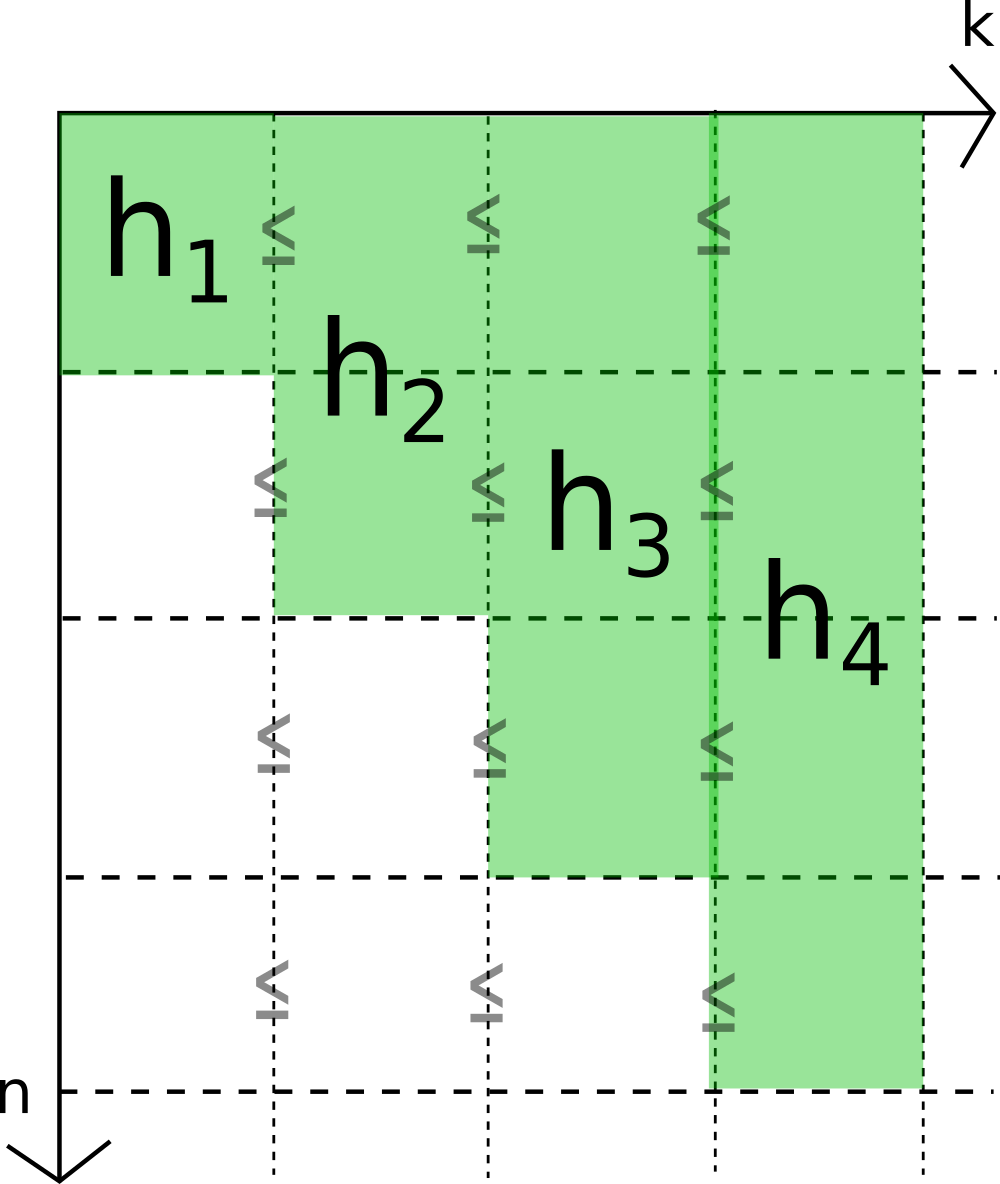
\includegraphics[width=0.25\textwidth]{mct_diagram.png}	
	\caption{Visualizing the definition $h_k$. Each square represents a $g_{n,k}$.}
\end{figure}
Notice that $h_1\leq h_2 \leq h_3 \leq \dots$ and $f=\lim_{k\to\infty}h_k$.
Hence
\[
	\int f \dm = \lim_{k\to\infty}\int h_k \dm \leq \lim_{n\to\infty}f_n \dm
\]
In generality, we can pick $N\in\mathcal{A}$ such that $\mu(N)=0$ and we have the assumed inequalities $\forall x\in N\stcmp$.
We can then apply these previous arguments to $N\stcmp$ by considering the functions
\[
	f\chi_{N\stcmp}, \quad f_1\chi_{N\stcmp} \leq f_2\chi_{N\stcmp} \leq f_3\chi_{N\stcmp} \leq \dots
\]
These functions differ on a set contained within a set of measure 0 and hence their integrals must agree with the full integrals.
\end{proof}
\begin{cor}[Levi's Theorem]
	Given measurable $g_n: X\to[0, +\infty]$ for each $n\in\N$.
	\[
		\int\left( \sum_{n-1}^{\infty}g_n \right)\dm = \sum_{n=1}^{\infty}\left(\int g_n \dm\right)
	\]	
\end{cor}
\begin{theorem}[Fatou's Lemma]
Given a sequence $\left\{f_n\right\}$ of functions in $\overline{S_+}$,
\[
	\int \left(\liminf_n f_n\right)\dm \leq \liminf_n \int f_n \dm
\]
\end{theorem}
\begin{proof}
For each $k\in\N$ define $g_k\defeq\inf_{n\geq k} f_n \in \overline{S_+}$.
\[
	g_1 \leq g_2 \leq g_3 \leq \dots \quad \text{and} \quad \liminf_n f_n = \lim_n g_n
\]
Apply the Monotone Convergence Theorem to see
\[
	\int \left(\liminf_n f_n \right)\dm = \int \left(\lim_n g_n\right)\dm = \lim_n \int g_n \dm
\]
So we need to show $\lim_n\int g_n \dm \leq \liminf_n \int f_n \dm$.
Notice for each $n\in\N$ that $g_n\leq f_n \leq f_{n+1} \leq \dots$ and hence
\[
\lim_n g_n \dm \leq \liminf_n \int f_n \dm
\]
\end{proof}
\begin{theorem}[Dominated Convergence Theorem]
Suppose:
\begin{enumerate}[label=(\roman*)]
	\item $g:X\to [0, +\infty]$ is integrable
	\item $f,f_1,f_2, \dots:X\to\Rb$ are measurable such that for almost every $x\in X$
		\[
			f(x) = \lim_{n\to\infty}f_n(x)\quad\text{and}\quad\forall n\in\N \;\abs{f_n(x)}\leq g(x)
		\]
\end{enumerate}
Then:
\begin{enumerate}
	\item $f$ and each $f_i$ are integrable
	\item $\int f \dm = \lim_{n\to\infty}\int f_n \dm$
\end{enumerate}
\end{theorem}
\begin{proof}
We may assume that \textit{(ii)} holds for every $x\in X$ since this won't change any integrals.
Likewise we may assume that $g(x)\neq + \infty$ for all $x\in X$.
\begin{enumerate}
	\item Given $n\in\N$, $\abs{f_n}\leq g\implies \int \abs{f_n} < \int g < + \infty \implies f_n \text{integrable}$.

		Then $\abs{f}=\lim_n\abs{f_n}\leq \lim_n g = g\implies f\text{integrable}$.
	\item \textbf{Claim: }$\int\left(g+f\right)\dm\leq\liminf_n\int\left(g+f_n\right)\dm$
		
		This follows by Fatou's Lemma because $g+f_n\geq 0$ is measurable and $g+f=\lim_n\left(g+f_n\right)$.
		Now,
		\begin{align*}
			\int g \dm + \int f \dm &= \int (g+f)\dm \\
									&\leq \liminf_n \left(\int \left(g+ f_n\right)\dm\right) \\
									&= \int g \dm + \liminf_n \int f_n \dm \\
			\text{and hence}\quad \int f \dm &\leq \liminf_n \int f_n \dm
		\end{align*}
		Now applying the same argument to $-f$ and $\left\{-f_n\right\}$ yields
		\[
			\int(-f)\dm \leq \liminf_n\int(-f_n)\dm \implies \int f \dm \geq \limsup_n \int f_n \dm
		\]
		And hence we have $\int f \dm = \lim_n \int f_n \dm$.
\end{enumerate}
\end{proof}
It's also worth knowing that
\begin{theorem}
Given bounded function $f:[a, b]\to\R$
\begin{enumerate}[label=(\alph*)]
	\item $f$ is Riemann integrable $\iff$ for almost every $x$, $f$ is continuous at $x$
	\item In this case Riemann Integral = Lebesgue Integral
\end{enumerate}
\end{theorem}
\end{document}
